\chapter{АНАЛИЗ ПРЕДМЕТНОЙ ОБЛАСТИ}
\aftertitle

\section{Постановка задачи кластеризации текста}

Кластеризация ~-- задача группировки объектов в подмножества, называемые кластерами, таким образом, чтобы объекты в одном кластере были больше похожи друг на друга, чем на объекты из других кластеров.

Задача кластеризации является одной из базовых задач машинного обучения и имеет большое количество практических применений в различных отраслях. Кластеризация может быть применима к объектам различного типа: кластеризация может быть применена к количественным или категориальным данным, изображениям, тексту и др.

Цель кластеризации текста состоит в том, чтобы автоматически разделить текстовые документы на группы (кластеры) с похожим содержанием. Это может быть полезно для большого количества задач, таких как организация большой коллекции текстовых документов, поиск похожих текстов или извлечение тем из текста.

Задача кластеризации текста активно изучается и применяется на протяжении многих лет. Кластеризация текста может иметь различные практические применения, таки как \cite{text-clustering-survey}:
\begin{itemize}
    \item поиск похожих документов;
    \item семантический поиск по коллекции документов;
    \item организация документов ~-- иерархическая организация документов в категории может быть полезна при систематическом исследовании коллекции документов;
    \item суммаризация текстов ~-- техники кластеризации могут быть применены для суммаризации коллекции документов, т.е. для сокращения объема текста, выделения ключевых слов и/или концепций;
    \itemк классификация документов ~-- техники кластеризация может быть использована для улучшения результатов классификации текстов в задачах обучения с учителем.
\end{itemize}

Кластеризация представляет собой задачу обучения без учителя. В процессе обучения, алгоритмы кластеризации самостоятельно определяют, какие существуют кластеры (в зависимости от алгоритма кластеризации, количество кластеров может быть задано вручную или же тоже быть определено и/или уточнено в процессе обучения) и на основе каких признаков относить объекты к тем или иным кластерам. Это делает кластеризацию полезной при работе с большим количеством данных, потому что устраняется необходимость в трудоемкой и дорогостоящей процедуре разметки данных. Это особенно актуально для задач обработки естественного языка, потому что позволяет использовать огромные объемы данных для обучения.

С кластеризацией тесно связана другая задача обработки естественного языка ~-- тематическое моделирование (англ. topic modeling). Тематическое моделирование ~-- способ построения модели коллекции текстовых документов, которая определяет, к каким темам относится каждый из документов. Это задача обучения без учителя, которая позволяет кластеризовать множество документов и соотнести кластерам их описание (слова, фразы), которые характеризуют документы в этом кластере. Иными словами, тематическое моделирование - это кластеризация, которая дополнительно определяет смысл и значение кластеров \cite{no-patterns}.

\section{Общая схема решения задачи кластеризации текста}

Чаще всего, задача кластеризации текста решается в два этапа:
\begin{enumerate}
    \item формирование эмбеддингов текстов, т.е. перевод текстов в векторное представление, которое может быть использовано в различных алгоритмах кластеризации;
    \item кластеризация полученных эмбеддингов с помощью тех или иных алгоритмов кластеризации.
\end{enumerate}

Тем не мене, существуют альтернативные подходы, которые предлагают end-to-end подход к кластеризации текста, используя общую нейронную сеть для выделения эмбеддингов и кластеризации [\cite{end-to-end-clustering}]. TODO: написать про метод и результаты.

\section{Способы получения эмбеддингов текста}

Для кластеризации текста в первую очередь необходимо произвести его векторизацию, т.е представить текст в виде эмбеддингов - векторов, которые могут быть далее использованы алгоритмами кластеризации. В обзоре \cite{no-patterns} выделяют три группы методов:
\begin{itemize}
    \item статические методы (классические);
    \item неглубокие (shallow) нейронные сети;
    \item глубокие нейронные сети, в частности, сети на основе механизма внимания.
\end{itemize}

\subsection{Статистические (классические) методы}

Наиболее простым классическим методом формирования эмбеддингов является мешок слов (Bag-of-Words, BoW). В этом методе, текст (предложение или весь документ) представляется в виде мультимножества, где каждому слову из текста сопоставляется количество или частота его вхождений. Для формирования мешка слов, составляется длинный вектор размерностью равной словарю, где каждое слово кодируется в виде one-hot вектора: выставляется 1 для текущего слова, и 0 для всех остальных слов. Вектора всех слов в документе можно суммировать для получения количественной информации о частоте встречаемости слов в документе. Модель мешка слов никак не учитывает грамматику, порядок слов в тексте и семантику, а учитывает только их количество.

Модификацией этого метода является метод Bag-of-n-grams. Вместо представления каждого слова независимо, в моделе представляются n-граммы (т.е. упорядоченные последовательности из n идущих подряд слов).

Согласно обзору \cite{no-patterns}, 19\% проанализированных статей использовали модели Bag-of-Words и Bag-of-n-grams.

Другим распространенным классическим методом является TF-IDF (TF — term frequency, IDF — inverse document frequency). Это статистическая мера, используемая для оценки важности слова в контексте документа, являющегося частью коллекции документов или корпуса. 30\% проанализированных статей использовали TF-IDF \cite{no-patterns}.

\subsection{Семантические эмбеддинги}

Следующая группа методов позволяют отражать эмбеддинги, учитывающие семантику языка. Они представляют текстовые данные в виде плотных векторов, которые отражают семантическую и синтаксическую связь между  объектами из похожих множеств. Эмбеддинги представляют слова в пространстве с меньшей размерностью, т.е. размерность векторов существенно меньше, чем количество слов. Такие эмбеддинги часто предобучены на большом корпусе текстов и публично доступны. Предобученные эмбеддинги часто используют в  topic modelling. Такие эмбеддинги обладают следующими свойствами
\begin{itemize}
    \item эмбеддинги семантически близких слов располагаются близко друг к другу (для оценки используется косинусное расстояние);
    \item похожие семантические отношения между словами описываются похожими векторами в пространстве эмбеддингов;
    \item можно проводить векторные операции над эмбеддингами; например, выражение "король - мужчина + женщина" будет приблизительно равно эмбеддингу слова "королева" \cite{word2vec};
    \item можно получать эмбеддинги фраз, складывая эмбеддинги составляющих их слов.
\end{itemize}

Визуализации семантических эмбеддингов на примере word2vec представлена на рисунке \ref{img:word2vec-demo}. На рисунке представлена проекция векторного представления слов в трехмерное пространство. Рисунок демонстрирует связи между словами. Стрелками отмечен вектор "man-king", отложенный от слова "man" (сверху) и от слова "woman" (снизу). Видно, что вектор "king - man + woman" наиболее близок к слову "queen".

\begin{figure}[h]
    \centering
    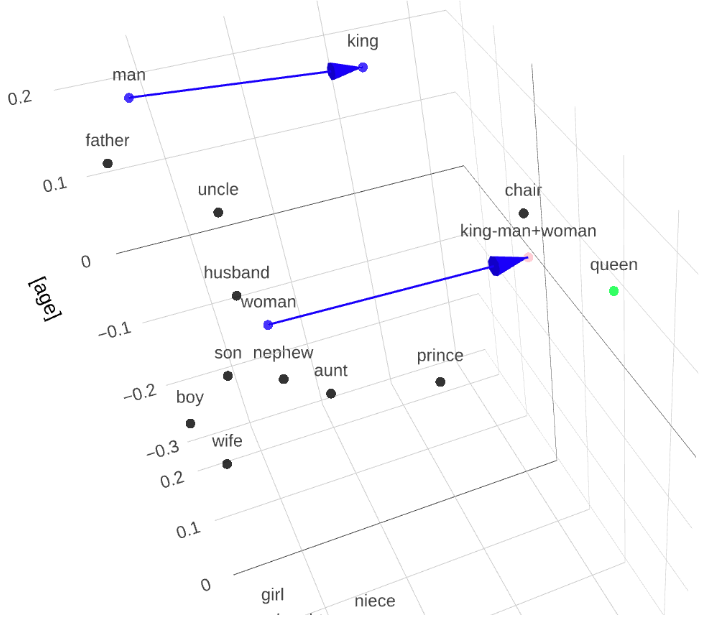
\includegraphics[width=\linewidth]{images/word2vec-demo.png}
    \caption{Визуализация word2vec \cite{word2vec-demo}}
    \label{img:word2vec-demo}
\end{figure}

Первым и наиболее известным подходом к построению семантических эмбеддингов является word2vec \cite{word2vec}. Этот метод позволяет представлять слова текста в виде векторов, близость (косинусное расстояние) которых отражает семантическую близость слов. Подход worc2vec основан на гипотезе локальности, которая утверждает, что слова, которые встречаются в одинаковых окружениях, имеют близкие значения. Это достаточно популярный способ создания эмбеддингов, 16\% проанализированных в работе \cite{no-patterns} статей используют word2vec.

Модель word2vec реализуется нейронной сетью прямого распространения (feedforward neural network) с одним скрытым слоем. Существует два подхода к построению модели word2vec: CBOW (continues bag of words) и skip-gram. В первом варианте модель обучается заполнять пропуски во фразах. На вход модели подаются два слова (в виде one-hot векторов), и модель предсказывает слово, которое располагалось между ними. Во втором случае модель, наоборот, обучается предсказывать контекст по данному слову.

Существуют другие варианты создания эмбеддингов, похожие на word2vec или являющиеся дальнейшим развитием заложенных идей: GloVe, fastText, doc2vec и другие \cite{no-patterns}, \cite{embeddings-habr}.

GloVe ~-- способ создание эмбеддингов, аналогично word2vec. Основное отличие GloVe от word2vec состоит в том, что в word2vec используется нейронная сеть, которая обучается предсказывать слова, расположенные рядом с целевым словом, в то время как GloVe использует статистику корпуса текста, чтобы обучить вектора слов \cite{glove}.

fastText ~-- способ создания эмбеддингов для частей слов. Модели, которые назначают эмбеддинг вектор целому слову, плохо работают с редкими словами  и словами, которые отсутствуют в корпусе. fastText решает эту проблему, путем обучения эмбеддингов для частей слов (n-grams) и затем составляя полный вектор эмбеддинга слова путем соединения векторов частей слова. fastText обучается с использованием подхода Skip-Gram. fastText показывает несколько худшие результаты, чем word2vec, но способен работать со незнакомыми словами. 4\% статей \cite{no-patterns} используют fastText;

doc2vec ~-- способ создания эмбеддингов не для отдельного слова, а для целого документа. 5\% статей \cite{no-patterns} используют doc2vec;

\subsection{Глубокие нейронные сети и контекстуальные эмбеддинги}

Проблемой семантических эмбеддингов является то, что они присваивают каждому слову из корпуса фиксированный эмбеддинг. Тем не менее, слова могут иметь различные значения, в зависимости от контекста, поэтому можно достичь большей точности в обработке текста, если генерировать эмбеддинги с учетом текущего контекста слова.

Первой моделью контекстуальных эмбеддингов стал ELMo \cite{elmo}. Эта модель обучается предсказывать следующее слово в предложении. Это так называемой задаче моделирования языка (language modeling). Для этого используется двунаправленная LSTM. Архитектура LSTM (long short-term memory) долгое время демонстрировала лучшие результаты в задачах обработки естественного языка и последовательностей. В качестве эмбеддинга слова выступает взвешенная сумма скрытых состояний LSTM.

В настоящее время лучшие результаты в задачах обработки естественного языка, в частности, в задачах кластеризации и тематического моделирования, показывают нейронные сети на базе архитектуры Transformer \cite{no-patterns}.

Трансформер представляет собой sequence-to-sequence модель, которая преобразует последовательность слов (токенов) на естесственном одном естесственном языке в другую последовательность слов на естесственном языке. Трансформеры могут применяться, к примеру, в задаче машинного перевода. Трансформер состоит из блока энкодеров и декодеров. Блок энкодеров состоит из последовательности идущих друг за другом энкодеров (стек энкодеров). Блок декодеров устроен аналогично. Каждый энкодер состоит из слоя self-attention и сети прямого распространения. Механизм внимания позволяет вес тех или иных частей последовательности и существенно улучшает результаты моделей \cite{transformer}.

В современных исследованиях в области обработки естественного языка активно применяется модель BERT и модели на ее основе. BERT (Bidirectional Encoder Representations from Transformers) ~-- языковая модель, основанная на архитектуре Transformer, предназначенная для предобучения языковых представлений [\cite{bert}].Архитектура BERT показана на рисунке \ref{img:bert-architecture}. BERT представляет собой обученный стек из двенадцати энкодеров трансформера.

На момент публикации, BERT показывал лучшие результаты в задачах обработки естественного языка, превосходя ранее существующие модели. BERT используется как энкодер, формируя эмбеддинги для токенов входного предложения. BERT применяется для различных задач, таких как задачи классификации (например, анализ тональности), определения похожести текстов и других. В частности, BERT может применяться и как эмбеддинги для задачи кластеризации \cite{text-clustering-with-bert}. В оригинальной работе предложен метод дообучения BERT как энкодера, таким образом, что выход CLS токена выступает в роле эмбеддинга. BERT обучается без учителя (self-supervised learning) на большом корпусе текстов с помощью метода masked language modeling, и дообучается для конкретной задачи (например, для задачи семантической классификации) с помощью обучения с учителем.

\begin{figure}[h]
    \centering
    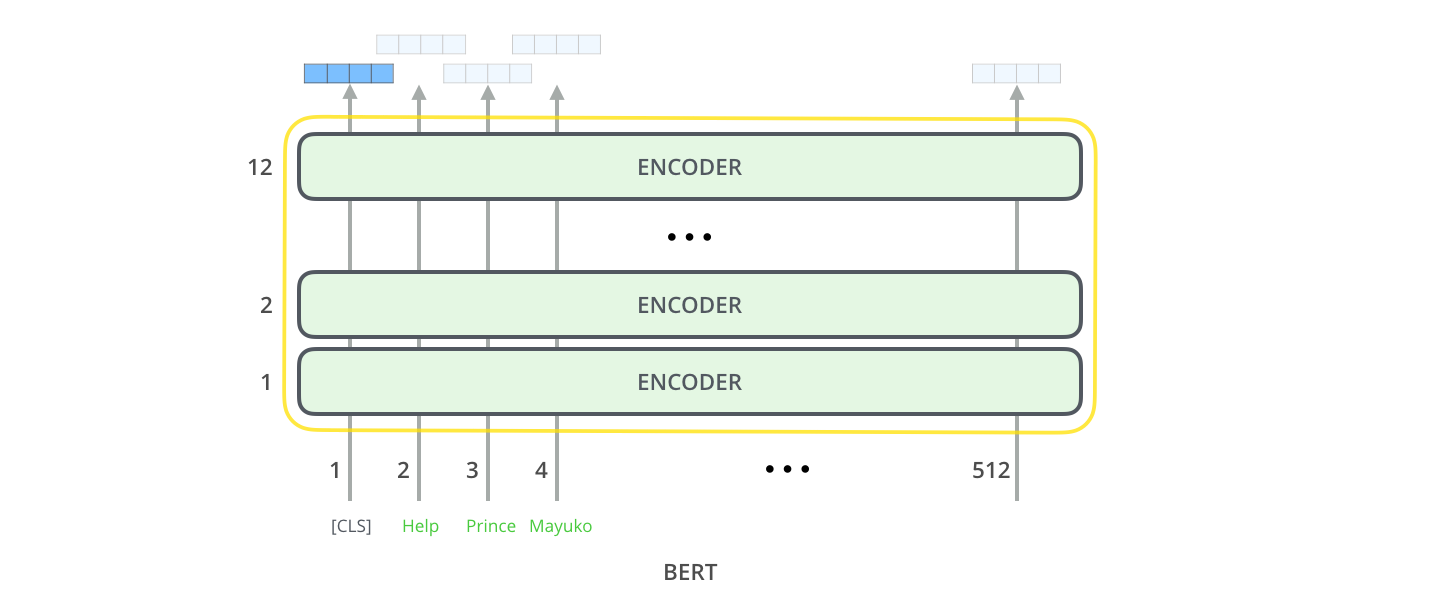
\includegraphics[width=\linewidth]{images/bert-architecture.png}
    \caption{Архитектура BERT}
    \label{img:bert-architecture}
\end{figure}

Рассмотрим некоторые современные модели, основанные на энкодерах трансформера и BERT \cite{mteb}. В основном, модели основаны на пред-обученном BERT и различаются механизмом дообучения. В различных моделях используются разные подходы для обучения без учителя и обучения с учителем на различных NLP-задачах:

% Так подробно расписывать каждую модель из статьи слишком долго, займет больше места, чем требуется на введение, а по итогу, слишком сжато и непонятно.
% В работе \cite{condenser} рассматриваются недостаток классического bidirectional transformer (таких, как BERT), заключающийся в том, что он неэффективно обучается объединению информации из всего предложения в токен CLS, потому что паттерны внимания таковы, что в большинстве слоев, этот токен мало задействуется. В этой работе предлагается модификация способа обучения Transformer, который позволяет лучше обучить модель собирать всю информацию о предложении в токен CLS. В результате, предложенный метод обучения модели, позволяет добиться лучших результатов, чем исходный BERT.
\begin{itemize}
    \item Consender ~--- архитектура, позволяющая более эффективного предобучать BERT-подобные модели с помощью добавления дополнительных слоев (т.н. condenser head) поверх исходной модели и дополнительного шага обучения без учителя перед дообучением на конкретной задаче \cite{condenser};
    \item Contriever ~--- модель, обученная с помощью дополнительного шага обучения без учителя (self-supervised learning) с использованием контрастного обучения (contrastive learning) для задачи извлечения текста;
    \item LaBSE ~--- модель для многоязычных эмбеддингов;
    \item SPECTER ~--- основывается на SciBERT (BERT, обученном на корпусе научных текстов) и дообучен на графах цитирования;
    \item GTR, ST5 ~--- модели, основанные на энкодерной части модели T5. T5 ~--- text-to-text модель энкодер-декодер, предобученная на нескольких NLP-задачах;
    \item Модели MPNEt и MiniLM обучались на разнообразном датасете, чтобы показывать хорошие результаты для любого применеия эмбеддингов.
\end{itemize}

TODO: В бенчмарке вообще не рассматриваются SBERT, ALBERT, RoBERTa и, быть может, еще какие-то модели, про которые я не знаю.

Также существуют модели на основе декодеров трансформера \cite{mteb}. Это различные варианты SGPT (Sentence embeddings for semantic search) на основе GPT-NeoX, GPT-J, BLOOM. Также в работе были рассмотрена модель cpt-text (трансформер для китайского языка) и OpenAI Embeddings API.

\subsection{Сравнение точности различных моделей для получения эмбеддингов}

В статье \cite{mteb} предлагается новый бенчмарк для тестирования эмбеддингов текста на различных задачах NLP. Обычно, точность эмбеддингов текста оценивают на ограниченном наборе задач, не рассматривая применения в других задачах. Таким образом, сложно отследить прогресс в развитии моделей и выбрать модель, обладающую лучшей  точностью для решаемой задачи. В статье решают эту проблему, представляя бенчмарк MTEB - Massive Text Embeddings Benchmark. Бенчмарк содержит восемь задач из области NLP, включая задачу кластеризации, состоит из 56 датасетов на 112 языках. В статье сравниваются 31 модель. Для сравнения в задаче кластеризации, модели использовались для получения эмбеддингов текстов, кластеризация осуществлялась с помощью метода k-means, в качестве метрики использовался v-measure.


На рисунке \ref{img:mteb_models} представлено сравнение точности (общей точности по всем задачам), производительности и размеров моделей, приведенных в исследовании \cite{mteb}.

\begin{figure}[h]
    \centering
    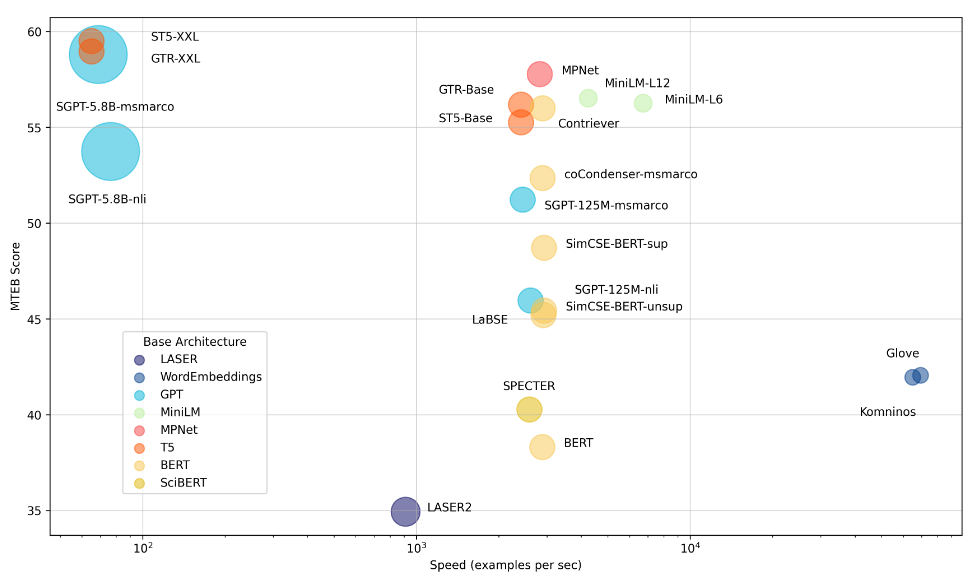
\includegraphics[width=\linewidth]{images/mteb-models.png}
    \caption{Сравнение точности, производительности и размеров моделей, приведенных в исследовании \cite{mteb}}
    \label{img:mteb_models}
\end{figure}

Результаты тестирования различных моделей в задаче кластеризации представлены в таблице \ref{tab:mteb}.

\begin{table}[ht]
    \caption{Сравнение моделей в задаче кластеризации \cite{mteb}}
    \label{tab:mteb}
    \begin{tabularx}{\textwidth}{|l|X|X|}
        \hline
        & Модель & V-Score \\
        \hline
        1 & ST5-XXL & 43.71 \\
        \hline
        2 & MPNet & 43.69 \\
        \hline
        3 & GTR-XXL & 42.42 \\
        \hline
        4 & MiniLM-L6 & 42.35 \\
        \hline
        5 & ST5-XL & 42.34 \\
        \hline
        6 & MiniLM-L12 & 41.81 \\
        \hline
        7 & GTR-Large & 41.6 \\
        \hline
        8 & GTR-XL & 41.51 \\
        \hline
        9 & Contriever & 41.1 \\
        \hline
        10 & SGPT-5.8B-msmarco & 40.35 \\
        \hline
        \multicolumn{3}{c}{...} \\
        \hline
        26 & BERT & 30.12 \\
        \hline
        \multicolumn{3}{c}{...} \\
        \hline
        29 & Glove & 27.73 \\
        \hline
        30 & Komninos & 26.57 \\
        \hline
        31 & LASER2 & 15.28 \\
        \hline

    \end{tabularx}
\end{table}

Большая часть представленных в исследовании моделей, кроме Glove, Komninos и LASER2 основаны на архитектуре Transformer. Модели Glove, Komninos ~--- это не-контекстуальные эмбеддинги (подобные word2vec, рассмотренному в предыдущем разделе). Они показывают худший результат, чем трансформеры, занимая последние места в таблице, но обладают существенно более высокой производительностью. Модель LASER2 является единственной моделью контекстуальных эмбеддингов, которая основана на LSTM, а не Transformer.

Несмотря на то, что модели ST5 и GTR имеют существенно больший размер и, соответственно, меньшую скорость работы, они незначительно опередили модели MPNet и MiniLM, которые практически в 50 раз меньше. Причиной этого может быть то, что MPNet и MiniLM дообучались на разнообразном датасете (для разных NLP-задач).


\section{Алгоритмы кластеризации}

TODO: написать подробнее про классификацию алгоритмов кластеризации из \cite{no-patterns}.
Кратко:
\begin{itemize}
    \item Representative-based clustering (k-means и похожие);
    \item Иерархическая кластеризация (HAC);
    \item Density-based clustering (DBSCAN).
\end{itemize}

В работе \cite{deep-clustering-survey} приводится обзор применения методов глубокого обучения для снижения размерности пространства признаков, чтобы алгоритмы кластеризации лучше справлялись с большими объемами данных с большим количеством признаков. Но эта статья не про кластеризацию текста, а в целом про кластеризацию. TODO: написать.

\section{Вывод}
TODO: написать вывод

TODO: Поместить эти статьи в подходящее место

В работе \cite{compare-text-clustering-sokolov} произведено сравнение следующих методов кластеризации текстовой информации: метод k-средних, алгоритм спектральной кластеризации, алгоритм агломеративной кластеризации и самоорганизующаяся карта Кохонена. В качестве данных использовалась коллекция новостей на русском языке. Для получения эмбедингов текста применялся алгоритм "мешок слов" ("bag of words"). В этой модели весь текст представлен одним вектором, хранящим информацию о количественном составе каждого слова в тексте. Недостатком данного подхода является отсутствие семантических связей между словами в тексте. В результате сравнения, алгоритмы показали достаточно близкую точность работы между собой, но, в среднем, самоорганизующиеся карты Кохонена оказались лучше других. Используемые алгоритмы сильно зависят от настройки гиперпараметров. Оптимальные параметры подбирались автоматически.

В работе \cite{method-text-clustering-andreev} дается обзор различных методов кластеризации, такие как: метод k-средних, suffix tree clustering, иерархические методы single link, complete link, group average, самоорганизующаяся карты Кохонена и сети ART (TODO: ???).
